\section{Motivation}

\begin{frame}[t]
	\frametitle{Motivation: Academic Interest}

	{\fontsize{10}{6}
		\begin{columns}
			\begin{column}{0.5\textwidth}
				\begin{itemize}
					\item Minimum jerk seems to be a thing
					      \begin{equation*}
						      \int_0^T \left\|\diffk{\qv}{t}{3}\right\| \d t
					      \end{equation*}
					      \begin{itemize}
						      \item Low frequency composition and  wear
						      \item Human-like motions accordint to Flash and Hogan
						      \item Psycological safety accoreding ...
					      \end{itemize}
					\item Minium Snap is of interest for drone motion planning
					      \begin{equation*}
						      \int_0^T \left\|\diffk{\qv}{t}{4}\right\| \d t
					      \end{equation*}
					\item Minium-X
				\end{itemize}
			\end{column}
			\begin{column}{0.5\textwidth}
				\begin{center}
					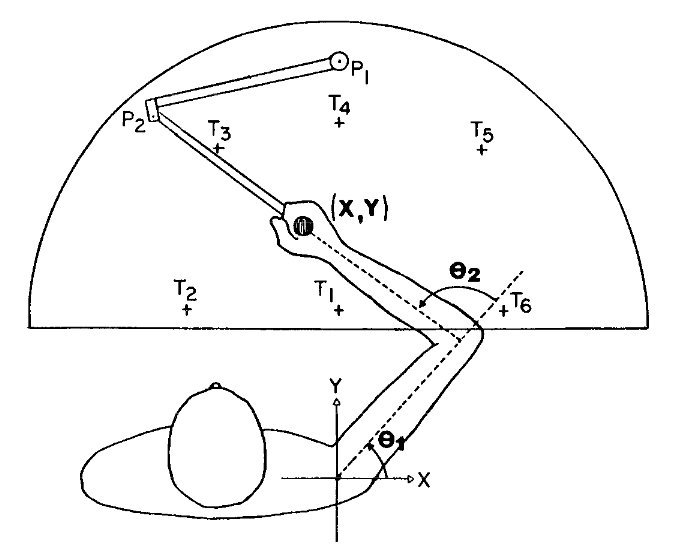
\includegraphics[width=0.4\textwidth]{./images/flashAndHoganExperiment.png}
				\end{center}
			\end{column}
		\end{columns}
	}
\end{frame}

\begin{frame}[t]
	\frametitle{Motivation: Output of Motion Planners}
	\begin{itemize}
		\item Sampled based planners generated waypoints
		\item Lead-Through/Hand-Guiding programming of cobots
		      \includemedia[
			      width=0.6\linewidth,   % Adjust width
			      height=0.4\linewidth,  % Adjust height
			      activate=onclick,      % Video starts on click
			      addresource=./images/cobotWaypoints.mp4, % Path to the video
			      flashvars={source=./images/cobotWaypoints.mp4&autoPlay=true&loop=true}
		      ]{}{VPlayer.swf}
	\end{itemize}
\end{frame}

\begin{frame}[fragile]
	\frametitle{Motivation: Current Classes Used in ROS Ecosystem}
	\begin{columns}
		\begin{column}{0.5\textwidth}
			\begin{itemize}
				\item Default ROS messages types for are defined as nested structrures.
				      The array-of-structures format leads to \emphImFusion{inefficient memory layout} and complicates the translation into the flat vector format that optimizers require.
				\item Other types are thighty coupled with the robot model
				\item do not provide clear interface for
				      \begin{itemize}
					      \item Evaluation at arbitrary time instantes
					      \item Computation of the derivatives
					      \item Time scaling
				      \end{itemize}
			\end{itemize}

		\end{column}
		\begin{column}{0.5\textwidth}
			Trajectory Message
			\begin{lstlisting}[basicstyle=\fontsize{5pt}{0pt}\selectfont\fontfamily{zi4}\selectfont]
std_msgs/msg/Header header
string[] joint_names
trajectory_msgs/msg/JointTrajectoryPoint[] points
            \end{lstlisting}
			Trajectory Point
			\begin{lstlisting}
double[] positions
double[] velocities
double[] accelerations
double[] effort
builtin_interfaces/msg/Duration time_from_start
                \end{lstlisting}
			Chomp trajectory
			\begin{lstlisting}
class ChompTrajectory
{
public:
...
    ChompTrajectory(const moveit::core::RobotModelConstPtr& robot_model, ...);
    double& operator()(size_t traj_point, size_t joint);
...
private:
...
    void init(); 
    std::string planning_group_name_;  
    Eigen::MatrixXd trajectory_;      
...
};
                \end{lstlisting}
		\end{column}
	\end{columns}
\end{frame}
